\documentclass[aspectratio=169]{beamer}

\usepackage{amsmath,amssymb}
\usepackage{graphicx}
\usepackage{tikz}
\usepackage{listings}
\usetikzlibrary{positioning,calc,arrows.meta,fit}

% =========================
% Colors
% =========================
\definecolor{PKUDarkPurple}{RGB}{63,63,191}
\definecolor{PKULightPurple}{RGB}{170,170,225}
\definecolor{PKUGrayBg}{RGB}{255,255,255}
\definecolor{PKUTextBlue}{RGB}{45,45,190}
\definecolor{CodeGray}{RGB}{245,245,245}
\definecolor{dkgreen}{rgb}{0,0.5,0}
\definecolor{gray}{rgb}{0.4,0.4,0.4}
\definecolor{mauve}{rgb}{0.58,0,0.82}

% =========================
% Global style
% =========================
\setbeamercolor{background canvas}{bg=PKUGrayBg}
\setbeamercolor{normal text}{fg=black,bg=PKUGrayBg}
\setbeamercolor{frametitle}{fg=PKUTextBlue,bg=PKUGrayBg}

\setbeamerfont{normal text}{size=\fontsize{15pt}{18pt}\selectfont}
\setbeamerfont{frametitle}{size=\fontsize{15pt}{19pt}\selectfont,series=\bfseries}
\setbeamerfont{itemize/enumerate body}{size=\fontsize{12pt}{15pt}\selectfont}
\setbeamerfont{itemize/enumerate subbody}{size=\fontsize{11pt}{14pt}\selectfont}
\setbeamerfont{footline}{size=\fontsize{10pt}{12pt}\selectfont}

\setbeamercolor{itemize item}{fg=PKUDarkPurple}
\setbeamertemplate{navigation symbols}{}
\setbeamertemplate{items}[ball]

\setbeamertemplate{headline}{}
\setbeamertemplate{footline}{}

% =========================
% Code style
% =========================
\lstset{
  basicstyle=\ttfamily\footnotesize,
  backgroundcolor=\color{CodeGray},
  keywordstyle=\color{blue},
  commentstyle=\color{dkgreen},
  stringstyle=\color{mauve},
  showstringspaces=false,
  breaklines=true,
  frame=single,
  columns=fullflexible
}

% =========================
% Custom headline
% =========================
\newcommand{\makecustomheadline}{
\begin{tikzpicture}[remember picture,overlay]
    \fill[PKUDarkPurple]
        (current page.north west)
        rectangle
        ([xshift=.50\paperwidth,yshift=-0.35cm]current page.north west);

    \fill[PKULightPurple]
        ([xshift=.50\paperwidth]current page.north west)
        rectangle
        ([xshift=\paperwidth,yshift=-0.35cm]current page.north west);
\end{tikzpicture}
}

% =========================
% Custom footline
% =========================
\newcommand{\makecustomfootline}{
\begin{tikzpicture}[remember picture,overlay]
    \fill[PKUDarkPurple]
        (current page.south west)
        rectangle
        ([xshift=.33\paperwidth,yshift=0.42cm]current page.south west);

    \fill[PKULightPurple]
        ([xshift=.33\paperwidth]current page.south west)
        rectangle
        ([xshift=.67\paperwidth,yshift=0.42cm]current page.south west);

    \fill[PKULightPurple]
        ([xshift=.67\paperwidth]current page.south west)
        rectangle
        ([xshift=\paperwidth,yshift=0.42cm]current page.south west);

    \node[anchor=center, text=white, font=\small]
        at ([xshift=.165\paperwidth,yshift=0.21cm]current page.south west)
        {\textrm{huangxun@pku.edu.cn}};

    \node[anchor=center, text=white, font=\small]
        at ([xshift=.50\paperwidth,yshift=0.21cm]current page.south west)
        {AI Enabled Control Engineering};

    \node[anchor=center, text=black, font=\small]
        at ([xshift=.83\paperwidth,yshift=0.21cm]current page.south west)
        {2026 Summer};

    \node[anchor=center, text=black, font=\small]
        at ([xshift=.965\paperwidth,yshift=0.21cm]current page.south west)
        {\insertframenumber/\inserttotalframenumber};
\end{tikzpicture}
}

\addtobeamertemplate{background}{\makecustomheadline\makecustomfootline}{}

% =========================
% Title info
% =========================
\title{\textcolor{PKUTextBlue}{AI Enabled Control Engineering}}
\author{\textcolor{blue}{Professor Xun Huang}}
\institute{
Aeronautics and Astronautics\\
College of Engineering\\
Peking University\\[0.25cm]
huangxun@pku.edu.cn\\
https://xunger99.github.io/xunger/
}
\date{}

\setbeamertemplate{title page}{
    \vspace{1.0cm}
    \begin{center}
        {\fontsize{18}{22}\selectfont\bfseries \inserttitle\par}
        \vspace{0.3cm}
        {\fontsize{15}{18}\selectfont Lecture 12: Hybrid Control, Sim-to-Real Improvement, and Final Demonstration\par}
        \vspace{0.3cm}
        {\fontsize{15}{18}\selectfont \insertauthor\par}
        \vspace{0.15cm}
        {\fontsize{11}{13}\selectfont TA: Zhixiang Ju \quad Haozhe Wang\par}
        \vspace{0.4cm}
        {\fontsize{8}{11}\selectfont \insertinstitute\par}
    \end{center}
}

\begin{document}

% ---------------------------------
\begin{frame}
\titlepage
\end{frame}

% ---------------------------------
\begin{frame}{Lecture 12 roadmap}
\begin{enumerate}
    \item Why hybrid control is needed for the rotary inverted pendulum.
    \vspace{0.18cm}
    \item Required hybrid schemes: DQN swing-up + MPC stabilization, and DQN swing-up + PPO stabilization.
    \vspace{0.18cm}
    \item Sim-to-real gap and residual-network correction idea.
    \vspace{0.18cm}
    \item Student design space: switching logic, residual usage, and safety rules.
    \vspace{0.18cm}
    \item Live demonstration assessment.
\end{enumerate}

\vspace{0.25cm}
\begin{block}{Class 12 goal}
\small
Students should design, test, compare, and demonstrate a hybrid control strategy for the real rotary inverted pendulum, and try to use a residual network to reduce the sim-to-real gap.
\end{block}
\end{frame}

% ---------------------------------
\begin{frame}{Why hybrid control?}

A single controller is usually not ideal for the whole RIP task.

\vspace{0.2cm}

\begin{itemize}
    \item Swing-up is a large-angle nonlinear task.
    \vspace{0.18cm}
    \item Upright stabilization is a local precision-control task.
    \vspace{0.18cm}
    \item DQN is suitable for learning a large-region discrete-action policy.
    \vspace{0.18cm}
    \item MPC is suitable for constrained local stabilization.
    \vspace{0.18cm}
    \item PPO may work well as a learned balancing controller near upright.
\end{itemize}

\vspace{0.2cm}

\begin{alertblock}{Main idea}
\small
Use different controllers in different regions of the state space.
\[
\text{large angle: swing-up policy}
\quad \Longrightarrow \quad
\text{near upright: stabilizing controller}
\]
\end{alertblock}

\end{frame}

% ---------------------------------
\begin{frame}{Hybrid control architecture}

\begin{center}
\resizebox{0.92\textwidth}{!}{
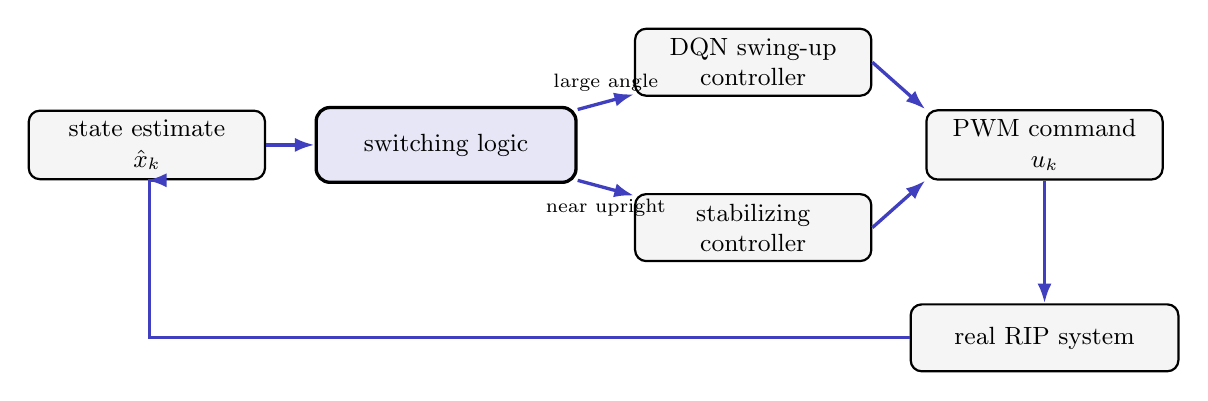
\begin{tikzpicture}[
    font=\small,
    >={Latex[length=2.5mm,width=1.8mm]},
    block/.style={
        draw,
        rounded corners=4pt,
        thick,
        align=center,
        minimum width=3.0cm,
        minimum height=0.85cm,
        fill=CodeGray
    },
    main/.style={
        draw,
        rounded corners=5pt,
        very thick,
        align=center,
        minimum width=3.3cm,
        minimum height=0.95cm,
        fill=PKULightPurple!30
    },
    arrow/.style={->, very thick, draw=PKUDarkPurple}
]

\node[block] (state) at (0,0) {state estimate\\$\hat{x}_k$};
\node[main] (logic) at (3.8,0) {switching logic};
\node[block] (swing) at (7.7,1.05) {DQN swing-up\\controller};
\node[block] (stab) at (7.7,-1.05) {stabilizing\\controller};
\node[block] (pwm) at (11.4,0) {PWM command\\$u_k$};

\draw[arrow] (state) -- (logic);
\draw[arrow] (logic) -- node[above] {\scriptsize large angle} (swing);
\draw[arrow] (logic) -- node[below] {\scriptsize near upright} (stab);
\draw[arrow] (swing.east) -- (pwm.north west);
\draw[arrow] (stab.east) -- (pwm.south west);

\node[block, minimum width=3.4cm] (plant) at (11.4,-2.45) {real RIP system};
\draw[arrow] (pwm.south) -- (plant.north);
\draw[arrow] (plant.west) -- ++(-9.65,0) |- (state.south);

\end{tikzpicture}
}
\end{center}

\vspace{0.15cm}

\begin{block}{Key design problem}
\small
The switching logic should avoid chattering, unsafe mode changes, and unstable handover between controllers.
\end{block}

\end{frame}

% ---------------------------------
\begin{frame}{Required hybrid scheme 1: DQN + MPC}

\begin{block}{Required experiment}
\small
Use DQN for swing-up and switch to MPC when the pendulum enters the upright region.
\end{block}

\vspace{0.2cm}

\begin{itemize}
    \item DQN handles large-angle nonlinear motion.
    \vspace{0.18cm}
    \item MPC handles local stabilization with PWM constraints.
    \vspace{0.18cm}
    \item Students should design the switching threshold and hysteresis.
    \vspace{0.18cm}
    \item The report should compare this hybrid controller with pure DQN deployment.
\end{itemize}

\vspace{0.2cm}

Example switching condition:
\[
|\alpha_k|<\alpha_{\mathrm{enter}},
\qquad
|\dot{\alpha}_k|<\dot{\alpha}_{\mathrm{enter}}.
\]

\vspace{0.05cm}

Example safety fallback:
\[
|\alpha_k|>\alpha_{\mathrm{exit}}
\quad \Rightarrow \quad
\text{return to DQN swing-up or stop safely}.
\]

\end{frame}

% ---------------------------------
\begin{frame}{Required hybrid scheme 2: DQN + PPO}

\begin{block}{Required experiment}
\small
Use DQN for swing-up and switch to PPO when the pendulum is close to upright.
\end{block}



\begin{itemize}
    \item DQN provides the global swing-up behavior.
    \vspace{0.18cm}
    \item PPO provides the learned local balancing policy.
    \vspace{0.18cm}
    \item The PPO controller should only be activated inside its reliable region.
    \vspace{0.18cm}
    \item Students should compare whether PPO or MPC gives better steady-state behavior.
\end{itemize}



\begin{alertblock}{Important}
\small
If the stabilizing controller does not include swing-up, students must not start it from the hanging-down position.
The DQN part is responsible for bringing the pendulum close to upright.
\end{alertblock}

\end{frame}

% ---------------------------------
\begin{frame}{Switching logic: avoid chattering}

A naive switch may repeatedly jump between two controllers.

\vspace{0.2cm}

Use hysteresis:
\[
\alpha_{\mathrm{enter}} < \alpha_{\mathrm{exit}}.
\]

\vspace{0.15cm}

For example:
\[
|\alpha|<15^\circ
\quad \Rightarrow \quad
\text{enter stabilization mode},
\]
\[
|\alpha|>25^\circ
\quad \Rightarrow \quad
\text{leave stabilization mode}.
\]

\vspace{0.15cm}

Also require a dwell time:
\[
|\alpha_k|<\alpha_{\mathrm{enter}}
\quad \text{for } N_{\mathrm{hold}} \text{ consecutive steps}.
\]

\vspace{0.1cm}



\end{frame}

% ---------------------------------
\begin{frame}[fragile]{Example switching pseudocode}

\begin{lstlisting}[basicstyle=\ttfamily\tiny]
if mode == DQN_SWINGUP:
    u = dqn_policy(state)

    if abs(alpha) < alpha_enter and abs(dalpha) < dalpha_enter:
        stable_counter += 1
    else:
        stable_counter = 0

    if stable_counter >= N_hold:
        mode = STABILIZE
        reset_stabilizer_if_needed()

elif mode == STABILIZE:
    u = stabilizer_policy(state)   # MPC or PPO

    if abs(alpha) > alpha_exit:
        mode = DQN_SWINGUP
        stable_counter = 0

u = saturate(u, -PWM_MAX, PWM_MAX)
\end{lstlisting}

\vspace{0.12cm}

\begin{alertblock}{Safety}
\small
If \(|\alpha|\), \(|\dot{\alpha}|\), or \(|\theta|\) exceeds the safety limit, stop the motor immediately.
\end{alertblock}

\end{frame}

% ---------------------------------
\begin{frame}{Sim-to-real gap}

A policy trained in simulation may fail on the real system.

\vspace{0.2cm}

Common reasons:
\begin{itemize}
    \item inaccurate friction and motor dead-zone model;
    \vspace{0.15cm}
    \item mismatch between simulated PWM and real motor torque;
    \vspace{0.15cm}
    \item sensor noise and angle calibration error;
    \vspace{0.15cm}
    \item delay and nonuniform sampling;
    \vspace{0.15cm}
    \item unmodeled mechanical vibration and loose wires.
\end{itemize}

\vspace{0.2cm}


\end{frame}

% ---------------------------------
\begin{frame}{Residual network idea}

The model predicts:
\[
x_{k+1}^{\mathrm{model}}
=
F_{\mathrm{model}}(x_k,u_k).
\]

The real system gives:
\[
x_{k+1}^{\mathrm{real}}.
\]

Define a residual:
\[
r_k
=
x_{k+1}^{\mathrm{real}}
-
x_{k+1}^{\mathrm{model}}.
\]

\vspace{0.12cm}

Train a residual network:
\[
\hat{r}_k
=
R_\phi(x_k,u_k).
\]

Then the corrected prediction becomes:
\[
x_{k+1}^{\mathrm{corr}}
=
F_{\mathrm{model}}(x_k,u_k)+R_\phi(x_k,u_k).
\]

\end{frame}

% ---------------------------------
\begin{frame}{How can the residual network be used?}

Students may freely design how to use the residual network.



Possible choices:
\begin{itemize}
    \item improve MPC prediction:
    \[
    x_{k+1}=F_{\mathrm{model}}(x_k,u_k)+R_\phi(x_k,u_k);
    \]

    \item correct the training simulation environment;

    \item generate an additional compensation term:
    \[
    u_k=u_{\mathrm{base}}+\Delta u_\phi;
    \]

    \item use it only for offline sim-to-real analysis.
\end{itemize}


\end{frame}

% ---------------------------------
\begin{frame}{Example 1: residual network for one-step MPC prediction}

The nominal discrete model used by linear MPC is
\[
x_{k+1}^{\mathrm{nom}}
=
A_d x_k+B_d u_k .
\]

\vspace{0.15cm}

The real hardware transition is approximated by the next estimated state:
\[
x_{k+1}^{\mathrm{real}}
\approx
\hat{x}_{k+1}.
\]

\vspace{0.15cm}

Define the one-step model residual:
\[
r_k
=
x_{k+1}^{\mathrm{real}}
-
x_{k+1}^{\mathrm{nom}} .
\]

\vspace{0.15cm}

Train a residual network:
\[
\hat r_k
=
R_\phi(\xi_k).
\]

Then the corrected prediction becomes
\[
x_{k+1}^{\mathrm{corr}}
=
A_d x_k+B_d u_k+R_\phi(\xi_k).
\]

\vspace{0.12cm}



\end{frame}


% ---------------------------------
\begin{frame}{Residual network input and output}

Use a short history window as the network input.



For example, with history length \(L=6\),
\[
\xi_k=
\left[
\hat{x}_{k-L+1},u_{k-L+1},
\hat{x}_{k-L+2},u_{k-L+2},
\ldots,
\hat{x}_{k},u_k
\right].
\]



Each step contains
\[
\hat{x}_k=
\begin{bmatrix}
\hat\theta_k&
\hat{\dot\theta}_k&
\hat\alpha_k&
\hat{\dot\alpha}_k
\end{bmatrix}^{\top},
\qquad
u_k .
\]



Therefore, the input dimension is
\[
L\times(4+1)=6\times5=30.
\]



The output is the four-dimensional one-step residual:
\[
R_\phi(\xi_k)
=
\begin{bmatrix}
d\theta_{\mathrm{res},k}\\
d\dot{\theta}_{\mathrm{res},k}\\
d\alpha_{\mathrm{res},k}\\
d\dot{\alpha}_{\mathrm{res},k}
\end{bmatrix}.
\]

\end{frame}



% ---------------------------------
\begin{frame}{Residual network improvement example}

The following table gives one example of validation-set improvement
for one-step prediction error.

\vspace{0.1cm}

\begin{center}
\renewcommand{\arraystretch}{1.22}
\begin{tabular}{c|c|c|c|c|c}
\hline
\(\boldsymbol{|\alpha|}\) range
& samples
& \(\theta\)
& \(\dot{\theta}\)
& \(\alpha\)
& \(\dot{\alpha}\) \\
\hline
\(0^\circ\)--\(2^\circ\)
& 25946
& 39.8\%
& 23.1\%
& 16.4\%
& 16.3\% \\
\hline
\(2^\circ\)--\(4^\circ\)
& 11741
& 41.0\%
& 25.6\%
& 19.2\%
& 19.2\% \\
\hline
\(4^\circ\)--\(6^\circ\)
& 3740
& 41.3\%
& 28.2\%
& 22.7\%
& 23.2\% \\
\hline
\(6^\circ\)--\(8^\circ\)
& 1065
& 46.8\%
& 32.1\%
& 26.5\%
& 27.1\% \\
\hline
\(8^\circ\)--\(10^\circ\)
& 246
& 46.6\%
& 35.6\%
& 32.0\%
& 33.3\% \\
\hline
All samples
& --
& 40.6\%
& 24.8\%
& 18.4\%
& 18.3\% \\
\hline
\end{tabular}
\end{center}


\begin{block}{Observation}
\small
The residual network reduces the nominal one-step prediction error.
The improvement becomes more significant when \(|\alpha|\) is larger, where the linear model mismatch is stronger.
\end{block}

\end{frame}



% ---------------------------------
\begin{frame}{How the residual enters MPC prediction}

Without residual correction:
\[
x_{k+1}=A_d x_k+B_d u_k.
\]

\vspace{0.15cm}

With residual correction:
\[
x_{k+1}=A_d x_k+B_d u_k+r_k.
\]

\vspace{0.15cm}

For a two-step prediction:
\[
x_{k+2}
=
A_d(A_d x_k+B_d u_k+r_k)+B_d u_{k+1},
\]
that is,
\[
x_{k+2}
=
A_d^2x_k+A_dB_du_k+B_du_{k+1}+A_dr_k.
\]

\vspace{0.15cm}

Thus the residual affects the future prediction sequence as
\[
r_k,\qquad A_dr_k,\qquad A_d^2r_k,\qquad \cdots .
\]

\vspace{0.12cm}


\end{frame}

% ---------------------------------
\begin{frame}{Why only one-step residual correction?}

\begin{columns}[T,totalwidth=\textwidth]

% ================= left column =================
\begin{column}{0.48\textwidth}

Theoretically, we may correct every predicted step:
\[
x_{k+i+1}
=
A_d x_{k+i}
+
B_d u_{k+i}
+
R_\phi(\xi_{k+i}).
\]

\vspace{0.15cm}

However, each residual-network inference adds computation latency.

\vspace{0.15cm}

In our real-time controller,
\[
T_s=5\,\mathrm{ms},
\qquad
f_s=200\,\mathrm{Hz}.
\]

\vspace{0.15cm}

If the residual network is evaluated many times inside the MPC horizon, the controller may exceed the \(5\,\mathrm{ms}\) control period.

\vspace{0.15cm}

\begin{alertblock}{Practical compromise}
\small
We only compute the residual correction once at the current step, and then propagate its effect through the prediction model.
\end{alertblock}

\end{column}

% ================= right column =================
\begin{column}{0.50\textwidth}
\vspace{-0.8cm}
\begin{center}
\includegraphics[width=1.1\textwidth]{delay.png}
\end{center}

\vspace{-0.1cm}

\begin{block}{Latency observation}
\small
Residual-corrected MPC increases the computation time by several hundred microseconds compared with pure MPC. This is still below \(5\,\mathrm{ms}\), but it reduces the real-time safety margin.
\end{block}

\end{column}

\end{columns}

\end{frame}

% ---------------------------------
\begin{frame}{What does the residual network learn?}

The residual contains several unmodeled effects:

\begin{itemize}
    \item friction and backlash;
    \vspace{0.12cm}

    \item PWM-to-torque mapping error;
    \vspace{0.12cm}

    \item parameter identification error;
    \vspace{0.12cm}

    \item sensor noise and delay;
    \vspace{0.12cm}

    \item local nonlinear dynamics not captured by the linearized model.
\end{itemize}

\vspace{0.2cm}

The training target is
\[
r_k=
x_{k+1}^{\mathrm{real}}
-
x_{k+1}^{\mathrm{nom}}.
\]

\vspace{0.15cm}

\begin{alertblock}{Important distinction}
\small
\(r_k\) is a one-step prediction residual, not the current state error.
In MPC, it should enter future prediction as an additive model correction.
\end{alertblock}

\end{frame}


% ---------------------------------
\begin{frame}{Example 2: offline model-reference adaptation idea}

A related idea is model-reference adaptation.

\vspace{-0.05cm}

Instead of directly correcting the next state prediction, it tries to make the real system behave like a chosen reference model.

\vspace{-0.05cm}
Reference model:
\[
x_{m,k+1}=f_m(x_{m,k})+g_m(x_{m,k})u_k.
\]

Real system with an input correction:
\[
u_{a,k}=u_k+\delta u_k.
\]

A neural network learns
\[
\delta u_k=T_\phi(x_{a,k},x_{m,k},u_k),
\]
so that the real system output follows the reference model output.
\vspace{-0.05cm}


\begin{block}{Offline version for our lab}
\small
Students can train \(T_\phi\) offline from hardware logs, then use it as a fixed compensation module during later experiments.
\end{block}

\end{frame}


% ---------------------------------
\begin{frame}{Reference from LipNet-MRAC}

The attached paper proposes a learning-based model-reference adaptive control method.

\vspace{0.15cm}

Its key ideas are:

\begin{itemize}
    \item use a neural network to adapt the input command;
    \vspace{0.12cm}

    \item make the real robot response close to a predefined reference model;
    \vspace{0.12cm}

    \item exploit a Lipschitz network to provide a stability-related condition;
    \vspace{0.12cm}

    \item demonstrate the method on a flying inverted pendulum experiment.
\end{itemize}

\vspace{0.15cm}

\begin{alertblock}{How we simplify it in this class}
\small
We do not require online LipNet adaptation.
Students may borrow the idea and train an offline residual or compensation network from logs.
The main grading focus remains the hybrid controller.
\end{alertblock}

\end{frame}




% ---------------------------------
\begin{frame}{Required experiments}

\begin{enumerate}
    \item DQN swing-up + MPC stabilization.
    \vspace{0.25cm}

    \item DQN swing-up + PPO stabilization.
    \vspace{0.25cm}

    \item Optional bonus schemes:
    \begin{itemize}
        \item DQN + LQR;
        \item DQN + residual-corrected MPC;
        \item pure RL policy with improved sim-to-real tuning;
        \item any safe hybrid strategy with better performance.
    \end{itemize}
\end{enumerate}

\vspace{0.15cm}

\begin{block}{Minimum requirement}
\small
Every group must complete and compare the two required hybrid schemes.
Additional successful schemes can be used for bonus discussion and live demonstration.
\end{block}

\end{frame}

% ---------------------------------


% ---------------------------------
\begin{frame}{Report requirements}

\begin{itemize}
    \item Describe the switching logic and thresholds.
    \vspace{0.15cm}
    \item Present DQN+MPC hardware control curves.
    \vspace{0.15cm}
    \item Present DQN+PPO hardware control curves.
    \vspace{0.15cm}
    \vspace{0.15cm}
    \item Compare \(\alpha(t)\), \(\theta(t)\), PWM, mode switching time, and stabilization duration.
    \vspace{0.15cm}
    \item Analyze sim-to-real mismatch.
    \vspace{0.15cm}
    \item Discuss whether residual-network correction helps, if used.
\end{itemize}

\vspace{0.15cm}

\begin{block}{Main grading focus}
\small
The report mainly evaluates hybrid control design, experimental comparison, and sim-to-real analysis.
\end{block}

\end{frame}

% ---------------------------------


% ---------------------------------
\begin{frame}{Final live demonstration}

At the end of the lab, each group will demonstrate its best controller on the real RIP system.

\vspace{0.2cm}

\begin{itemize}
    \item Each group selects one best-performing scheme.
    \vspace{0.18cm}
    \item The controller should be started under the correct condition.
    \vspace{0.18cm}
    \item The group should briefly explain the controller structure and switching rule.
    \vspace{0.18cm}
    \item The experiment will be judged by actual control performance and safety.
\end{itemize}

\vspace{0.2cm}

\begin{block}{Live assessment}
\small
The live demonstration is the closing assessment of the RIP experiment series.
A successful demonstration should show stable control and clear understanding of the hybrid strategy.
\end{block}

\end{frame}

% ---------------------------------
\begin{frame}{Final demo scoring guideline}

\begin{center}
\begin{tabular}{c|p{0.68\textwidth}}
\hline
\textbf{Item} & \textbf{Criterion} \\
\hline
Safety & Correct start procedure, no unsafe motor behavior, emergency stop ready. \\
\hline
Hybrid logic & Clear mode switching, no severe chattering, reasonable thresholds. \\
\hline
Control effect & Successful swing-up and stable upright behavior. \\
\hline
Data quality & Logs and plots are complete, including mode and PWM. \\
\hline
Explanation & Group can explain why the method works or fails. \\
\hline
Bonus & Residual correction or other creative hybrid strategy improves performance. \\
\hline
\end{tabular}
\end{center}

\end{frame}

% ---------------------------------
\begin{frame}{Summary of the final lab}

\begin{itemize}
    \item Hybrid control combines the strengths of different controllers.
    \vspace{0.2cm}
    \item DQN can be used for large-angle swing-up.
    \vspace{0.2cm}
    \item MPC or PPO can be used for upright stabilization.
    \vspace{0.2cm}
    \item Residual networks provide one possible way to reduce sim-to-real mismatch.
    \vspace{0.2cm}
    \item The final goal is not only to run code, but to design, test, compare, and explain a complete control strategy.
\end{itemize}

\vspace{0.2cm}

\begin{alertblock}{Take-home message}
\small
AI-enabled control is an engineering loop:
modeling, simulation, learning, deployment, logging, diagnosis, and redesign.
\end{alertblock}

\end{frame}

\end{document}
